% ============================================================
% Red team / environment relationship (closed loop)
% Compile with:  pdflatex red_team_env.tex
% Output:        red_team_env.pdf
% ============================================================
\documentclass[border=4pt]{standalone}
\usepackage{tikz}
\usetikzlibrary{shapes.geometric, arrows.meta, positioning, fit, backgrounds, calc}

\definecolor{colAttack}{RGB}{245,225,225}
\definecolor{colReal}{RGB}{245,235,215}
\definecolor{colObs}{RGB}{220,235,245}
\definecolor{colDef}{RGB}{220,245,220}
\definecolor{colBorder}{RGB}{80,100,120}
\definecolor{colArrow}{RGB}{60,80,100}

\tikzset{
  box/.style={
    rectangle, rounded corners=3pt,
    draw=colBorder, line width=0.7pt,
    text centered, font=\small,
    inner sep=5pt, minimum height=1.8em
  },
  attackBox/.style={box, fill=colAttack, minimum width=3.2cm, minimum height=1.6cm, align=center},
  realBox/.style={box, fill=colReal, minimum width=3.2cm, minimum height=1.6cm, align=center},
  obsBox/.style={box, fill=colObs, minimum width=3.2cm, minimum height=1.6cm, align=center},
  defBox/.style={box, fill=colDef, minimum width=3.2cm, minimum height=1.6cm, align=center},
  arr/.style={
    -{Stealth[length=5pt]}, line width=0.8pt, color=colArrow
  },
  label/.style={font=\footnotesize, text=colBorder}
}

\begin{document}
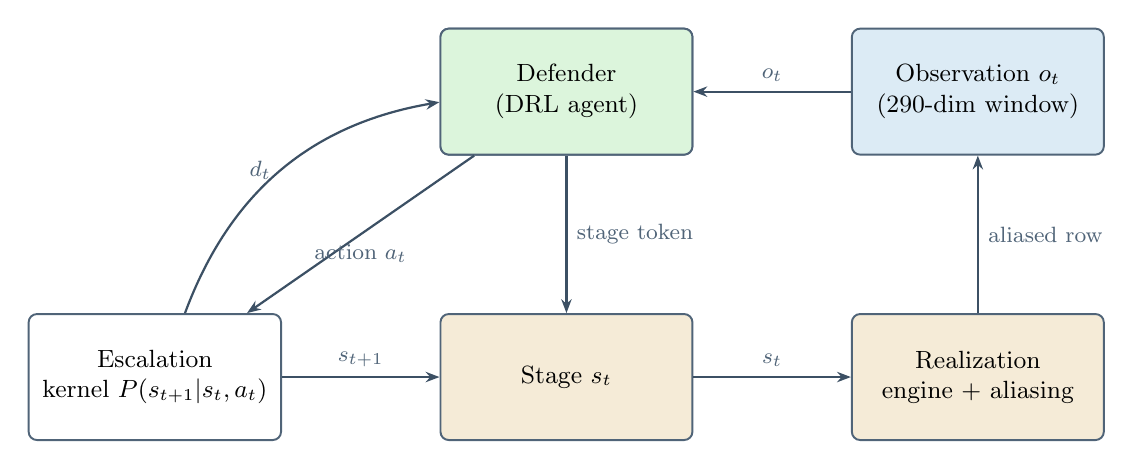
\begin{tikzpicture}[node distance=2.0cm]

  \node[attackBox] (attacker) {Reactive escalation\\attacker};
  \node[realBox, below=of attacker] (stage) {Stage $s_t$};
  \node[realBox, right=of stage, node distance=3.2cm] (real) {Realization\\engine + aliasing};
  \node[obsBox, above=of real] (obs) {Observation $o_t$\\(290-dim window)};
  \node[defBox, left=of obs, node distance=3.2cm] (defender) {Defender\\(DRL agent)};
  \node[box, left=of stage, node distance=3.2cm, minimum width=3.2cm, minimum height=1.6cm, align=center] (kernel) {Escalation\\kernel $P(s_{t+1}|s_t,a_t)$};

  % attacker emits stage
  \draw[arr] (attacker) -- node[label, right] {stage token} (stage);

  % stage -> realization
  \draw[arr] (stage) -- node[label, above] {$s_t$} (real);

  % realization -> observation
  \draw[arr] (real) -- node[label, right] {aliased row} (obs);

  % observation -> defender
  \draw[arr] (obs) -- node[label, above] {$o_t$} (defender);

  % defender -> kernel (action)
  \draw[arr] (defender) -- node[label, below] {action $a_t$} (kernel);

  % kernel -> stage (next stage)
  \draw[arr] (kernel) -- node[label, above] {$s_{t+1}$} (stage);

  % kernel -> attacker (d_t feedback)
  \draw[arr] (kernel) to[bend left=30] node[label, left] {$d_t$} (attacker);

\end{tikzpicture}
\end{document}
